\documentclass[11pt]{article}
\usepackage[T1]{fontenc}
\usepackage{lmodern}
\usepackage[margin=0.95in]{geometry}
\usepackage{amsmath,amssymb,amsthm,booktabs,longtable,array,graphicx}
\usepackage{microtype,enumitem,xcolor}
\usepackage[hidelinks]{hyperref}
\usepackage{listings}
\definecolor{teal}{HTML}{126B76}
\definecolor{muted}{HTML}{46556A}
\lstset{basicstyle=\small\ttfamily,breaklines=true,columns=fullflexible,
  keepspaces=true,frame=single,rulecolor=\color{black!15},xleftmargin=3pt,xrightmargin=3pt}
\setlist{itemsep=3pt,topsep=5pt}
\setlength{\emergencystretch}{2em}
\newtheorem{theorem}{Theorem}
\newtheorem{lemma}[theorem]{Lemma}
\newcommand{\Con}{\operatorname{Con}}
\newcommand{\Halt}{\operatorname{Halt}}
\newcommand{\N}{\mathbb N}
\newcommand{\file}[1]{\texttt{\detokenize{#1}}}
\title{\textbf{Rebalancing a 215-State ZFC Consistency Machine}\\[5pt]
  \large An exact transition table, a source bisimulation,\\
  and further routes toward 214 states}
\author{Research packet prepared for the ProveIt repository\\
  \small Construction, symbolic verification, and independent finite review}
\date{21 October 2026}
\begin{document}
\maketitle
\begin{abstract}
We construct K215-R41, a binary Turing machine with 215 working states,
whose blank-tape nonhalting is equivalent in ZFC to $\Con(\mathrm{ZFC})$
at the ordinary mathematical proof level of the repository's accepted K215.
Ten physically realizable reassociations of closed source factors change
19 transition rows and 4,120 instruction addresses. Maximum address depth
decreases from 47 to 41; total address length decreases by 6.8869\%.
The new rooted transition graph is not a renaming of any of the three
accepted 215-state graphs examined. The full 6,176-case arbitrary-natural
runtime check passes, as does an independent replay of the exact
95,714-step blank initialization. This is a different 215-state encoding,
not a 214-state construction or a uniform runtime speedup.

The packet also records a source with maximum zero run five, an
experiment replacing freshness rejection by matrix inflation, and two
instructive interpreter/initialization mismatches. The matrix-inflation
experiment removes thirteen primitive occurrences but has an explicit
unresolved native-calculus consistency bridge. Its status is research,
not a second certified consistency machine. Reproduction scripts, literal
tables, full source, runtime records, and this manuscript are included.
\end{abstract}

\section{Result and exact scope}
\label{sec:result}

The completed result is the second option in the request: a materially
different 215-state machine. The accepted reference is ProveIt's primary
\file{candidate-k215}, pinned at commit
\begin{center}\small\ttfamily
75716498437bfc7291d5900cab2983a11fd54bac.
\end{center}
All comparisons in this report refer to this immutable snapshot, not to
whatever the repository's main branch may contain later. The relevant
ordinary proof and source-calibration documents are included under
\file{baseline/}; their upstream locations are listed in the references.

\begin{center}
\begin{tabular}{lrr}
\toprule
Quantity & Primary K215 & K215-R41\\
\midrule
Working states, excluding halt & 215 & 215\\
Binary transition rows & 430 & 430\\
Distinct source subtrees & 202 & 202\\
Primitive occurrences & 4,751 & 4,751\\
Guarded primitive cases & 6,176 & 6,176\\
Maximum source-address depth & 47 & \textbf{41}\\
Sum of source-address lengths & 160,305 & \textbf{149,265}\\
Maximum zero run in a source address & 6 & 6\\
Blank initialization transitions & 95,714 & 95,714\\
\bottomrule
\end{tabular}
\end{center}

\begin{theorem}[Exact-table claim, with inherited logical calibration]
Let $M$ be the literal dense table in \file{machine/k215r.tm}, with
start state 0, binary blank symbol 0, and separate halt state 215.
The accepted K215 numerical-calculus calibration, the source
bisimulation established here, the complete symbolic primitive
contracts, and the exact blank prefix compose into an ordinary proof
formalizable in ZFC of
\[
 \Halt(M,\mathrm{blank})\ \longleftrightarrow\ \neg\Con(\mathrm{ZFC}).
\]
Consequently ZFC proves
\[
 \neg\Halt(M,\mathrm{blank})\ \longleftrightarrow\ \Con(\mathrm{ZFC}).
\]
\end{theorem}

The statement uses the usual syntactic consistency sentence: there is
no finite ZFC refutation in the calibrated proof coding. It does not
assert that ZFC proves either side individually. The new work changes
the encoding; it reuses the existing compact-calculus consistency
reduction. No new Lean or Rocq kernel endpoint, or internal-PA proof
certificate for this exact table, is claimed. The executable symbolic
checker is an ordinary mathematical induction checker.

\section{Literal machine and file identities}

The tape is two-way infinite, indexed by $\mathbb Z$, and initially
all zero. The head starts at coordinate zero. Every working state has
one transition for each read symbol in $\{0,1\}$, writing a bit and
moving exactly one cell left or right. There are no stationary moves,
extra tape symbols, or external input. Initialization is included in
the 215 states.

Each noncomment line of either table is
\begin{center}\file{state read write direction next-state}.\end{center}
The native presentation preserves upstream labels: start 0,
dispatcher 84, halt 254. Its labels are sparse; their maximum is not the
state count. The dense presentation uses breadth-first numbering from
start 0, reading the 0-edge before the 1-edge. Its working states are
exactly $0,\ldots,214$, dispatcher 23, halt 215. The explicit bijection
is in \file{machine/canonicalization.json}.

The following SHA-256 identities fix the result:
\begin{description}[style=nextline,leftmargin=0pt,labelwidth=0pt,labelsep=0pt]
\item[\file{machine/k215r.native.tm}]
\mbox{\small\ttfamily 8cfb95be77f8f8819ac7dc5c92297cf32b5104cbdf22aea925ab38de9c4443b9}
\item[\file{machine/k215r.tm}]
\mbox{\small\ttfamily 27a2a4f452f9fcb1e84ba6f78d0f952ea438eca00d415cc6b0ef4298d35086a4}
\item[\file{machine/sites215r.json}]
\mbox{\small\ttfamily 46ab3fdabc6ade3c6e4b5f08a0a59af66eb96f3992124ab6b71b8c3f1a05bf35}
\end{description}

Rooted canonical transition graphs retain the read label, written bit,
move direction, distinguished start, and halt. The canonical graph of
K215-R41 differs from each of the primary, commands120, and composed
215-state graphs in the pinned repository. The source164 alternative is
an exact renaming of composed and is thereby covered. This proves
distinctness under state renaming; it is not a claim that no more
general tape or computation conjugacy exists.

\section{Construction idea: rebalance the physical decoder}
\label{sec:construction}

An abstract source tree can be reassociated cheaply, but a smaller or
shallower abstract tree need not admit a binary-state allocation of the
same size. States may serve both source decoding and arithmetic-engine
roles. A source-only optimizer therefore has the wrong cost model if it
counts only distinct subtrees. Our successful search operates on source
and physical decoder together. It accepts a rotation only when its
actual existing states can implement the changed tree.

\subsection{Source semantics and the safe equivalence}

The source is a full binary tree whose leaves are instructions over nine
natural registers. In ordinal order there are 4,751 leaves. A leaf is
an increment $\mathrm{CI}_i$, a guarded decrement $\mathrm{CD}_i$, a
break $\mathrm{CB}_k$, a continue $\mathrm{CC}_k$, or halt.
Ordinary sequential motion goes to the next leaf, with root wraparound.
For decrement zero, the control exits the nearest ancestor at which
the current subtree is a left child; for positive decrement it reduces
the register and goes to the next leaf. A depth-$k$ break exits the
$k$th such left-child ancestor; a depth-$k$ continue restarts the
$k$th right-child ancestor. The included two graph resolvers specify
these rules independently by address arithmetic and subtree intervals.

A factor is \emph{closed} when it contains no halt and every break,
zero-decrement exit, or continue demand is discharged within the factor,
allowing its ordinary return boundary. The inherited
boundary calculation returns $(0,0,\mathrm{false})$ for every factor
used here. For such $A,B,C$, the reassociation
\[
               (A,(B,C))\quad\longleftrightarrow\quad((A,B),C)
\]
preserves execution order, register effects, normal return, and
divergence. Internal depth operands do not acquire different external
targets: every nonlocal control demand is discharged within the factor,
and an exit caught at its root is its ordinary return.

The construction checks a stronger global statement after every move:
the ordered opcode/operand word and the entire guarded ordinal
control-flow graph are unchanged. The graph has 6,175 successor edges
and one halt case. Both independent graph resolvers agree on the
reference and transformed source. Thus
\[
 (\text{old ordinal},r_0,\ldots,r_8)
 \quad\mathrel{\sim}\quad
 (\text{same new ordinal},r_0,\ldots,r_8)
\]
is a step-for-step source bisimulation. It holds for all natural
register values, including arbitrary undecodable formula codes. No
finite sample of register values is needed for this source conclusion.

\subsection{A four-row decoder rotation}

Suppose states $q,m$ are pure binary decoder states: on each read bit
they preserve that bit and move right. A left rotation replaces
\[
\begin{array}{c|cc}
 &0&1\\\hline
q&a&m\\m&b&c
\end{array}
\qquad\text{by}\qquad
\begin{array}{c|cc}
 &0&1\\\hline
q&m&c\\m&a&b
\end{array}
\tag{R}
\]
where the entries denote next states. It implements
$(A,(B,C))\mapsto((A,B),C)$ without adding a state; the right rotation
is its inverse. The checked side conditions require unique source roles
for these states and a private internal child $m$ at that parent
occurrence. Every resulting internal decoder prefix is then replayed
from the actual dispatcher with its known tape prefix restored exactly.

These local decoder facts are not an all-tape equivalence theorem for
the two complete machines: program-counter encodings change. The new
full runtime check in Section~\ref{sec:runtime} is necessary precisely
because existing labels can have other roles in the engine.

\subsection{The ten rotations}

The deterministic recipe is short. Native state labels are used in
Table~\ref{tab:recipe}; factor sizes are counts of primitive occurrences
at the instant of that rotation. Every selected parent has one source
occurrence in this recipe.

\begin{table}[htbp]
\centering
\begin{tabular}{rrrrrrr}
\toprule
Step & Parent $q$ & Child $m$ & Direction & $|A|$ & $|B|$ & $|C|$\\
\midrule
1&203&101&left &503&401&2,778\\
2&223&132&right&919&123&1,028\\
3&203&204&left &904&56&2,722\\
4&177&203&right&960&2,722&103\\
5&203&215&right&2,070&652&103\\
6&203&223&right&919&1,151&755\\
7&181&177&right&960&2,825&134\\
8&188&181&left &189&960&2,959\\
9&204&101&right&503&401&56\\
10&142&143&left&27&67&52\\
\bottomrule
\end{tabular}
\caption{The complete simplified construction. Left means (R); right means its inverse.}
\label{tab:recipe}
\end{table}

The search history initially contained fourteen rotations. Two pairs of
inverse operations commute with intervening moves. Deleting their four
members gives the ten-step recipe, with byte-identical final source,
native table, and dense table. Both recipes are preserved; the default
constructor and independent reviewer use the ten-step one.

\section{Complete runtime and calibrated blank input}
\label{sec:runtime}

Source equivalence alone does not establish a result for a blank binary
machine. Two further obligations were discharged on the exact frozen
table: arbitrary-natural primitive execution and complete blank
initialization.

\subsection{What the symbolic checker proves}

The unchanged inherited checker \file{runtime/runtime/symbolic_runtime.py}
uses literal machine transitions together with unary-scan induction and
finite-list induction. It rederives four one-block list schemas from
the supplied transition table. For each source occurrence and each
applicable decrement guard, it proves a whole-tape block from the
represented source frame to the next represented frame, or to halt at
the source halt. Registers and padding are symbolic natural numbers;
the spare list has arbitrary positive finite length and arbitrary
natural entries. The complete exterior is zero, rather than unspecified.

The frame convention has logical registers
$[N,T,W,A,D,H,X,Y,L]$, whose physical block indices are
$(6,2,0,4,3,7,8,5,1)$. Each unary value $v$ uses a block of $v+1$
ones with its prescribed zero separator. At the root the 64-position
program-counter field starts at the head and is followed by an arbitrary
natural gap, then the header and register/spare blocks. The checker accounts for
the exact program-counter word at every source occurrence, rather than
assuming that a shallower tree automatically has the same encoding.

The fresh completed run reports:
\begin{center}
\begin{tabular}{lr}
\toprule
Guarded cases expected / proved & 6,176 / 6,176\\
Failed cases & 0\\
Symbolic rules used & 1,640,317\\
Minimum affine duration constant & 6\\
Literal transition rows covered & 430 / 430\\
\bottomrule
\end{tabular}
\end{center}

Every recorded duration has positive constant term and nonnegative
coefficients. Each represented natural frame therefore executes its
primitive in a finite positive number of transitions. This makes the
simulation valid both for halting and for infinite source computation.
A finite symbolic-construction cap is a cap on the proof search, not on
register values, spare-list length, or actual represented running time.

The full receipt, every case record, four schema traces, checker source,
helper source, and native-label mapping are delivered. The independent
review audits those actual receipts, checks their input/code identities,
case order, guards, positive affine clocks, and complete row coverage.
It also replays the four block traces on the literal table. It does not
pretend to be a second implementation of the entire induction checker.

\subsection{The complete 95,714-step prefix}

Starting from the all-zero tape in state 0, the new table reaches exactly
the accepted source root after 95,714 transitions:
\[
\begin{gathered}
q=84,\qquad h=-8,\qquad \text{header}=57,\qquad\text{gap}=1,\\
[N,T,W,A,D,H,X,Y,L]=[4,0,0,0,0,0,0,0,0],\\
\text{forty spare blocks, each of value one.}
\end{gathered}
\]
The tape has exactly 95 one-cells and is zero everywhere else. The root
verifier constructs this expected complete frame independently and
executes the table literally for all 95,714 steps. The independent
review separately replays every saved transition and compares the
complete final support. The source's formula-bearing top, cache, and
stack are all zero. The nonzero enumeration counter four is permitted
by the cofinal completeness argument below.

\section{Why the exact machine still searches for a ZFC refutation}
\label{sec:logical}

The inherited numerical calculus is intentionally more permissive than
a literal well-formed first-order parser. Write
\[
 P(a,b)=\frac{(a+b)(a+b+1)}2+b,\qquad
 I(a,b)=4P(a,b),\qquad Q_i(a)=4P(i,a)+2.
\]
Truth is 0 and falsity is 1. The equality $I(0,0)=0$ is a real alias,
not an encoding error to be removed. Axiom instances and proof commands
operate on raw natural codes, including junk. The inherited calibration
shows that derivability of code 1 is equivalent to a finite ZFC
refutation; faithful first-order decoding of every intermediate code is
not a required invariant.

The accepted fragment uses seven logical rows, the permitted theory
bundle, numerical modus ponens, theorem-only generalization, and
\[
 \rho_8(A,B,C,U)=((C\to U)\to A)\to((A\to C)\to(B\to C)),
 \qquad U\leq A.
\]
A previously supplied 3,728-node finite derivation recovers the
unrestricted row at every raw numerical instance. Numerical implication
dominates its components, making the admissible substitution contexts
valid even when zero aliases collapse. Replacing each unrestricted
axiom by its fixed derived proof preserves exact theorem numerals and
the coupled theory bundle. That predecessor logical result is reused
here, not re-proved by our source graph checks \cite{dominated}.

For clarity, the command-calibration theorem can be separated into
soundness and completeness \cite{permuted}. At a boundary, top, cache,
and every decoded stack head are theorem codes. Numerical MP preserves
this invariant, the AX command introduces permitted instances, and the
stack commands move existing codes. NIP halts only upon testing code 1.
Starting with truth in top/cache and a zero stack is sound, including
the infinite truth tail arising from $P(0,0)=0$.

For completeness, the accepted strong compiler maps a finite derivation
of a code $X$ to a finite command block which, from a boundary with
counter and cache zero, either halts earlier or returns $X$ on the
original stack with counter and cache reset. Explicit
blocks handle row selection, MP, and GEN, including zero aliases.
A block for 1 is followed by the finite halt-testing suffix. Nonhalting
candidate proof lists drain, so malformed candidates cannot permanently
block enumeration. The command tags are NIP 0, DROP 1, MP 2, and AX
$c+3$, with the accepted YX field order.

The cofinal construction is necessary because the actual blank seed
starts at candidate four. If $R$ encodes a fixed refutation block,
prefixing the accepted resetting AX command gives candidate numbers
\[
                P(3,P(Y,P(1,R)))\ \geq\ Y.
\]
Thus a successful candidate exists beyond every finite cutoff; in
particular one exists beyond four whenever the calculus is inconsistent.
Both directions apply to the exact seed in Section~\ref{sec:runtime}.

The new source has precisely the same ordinal/register transition
system. The proof chain for the frozen binary table is therefore
\[
\begin{aligned}
\Halt(M,\mathrm{blank})
&\iff \Halt(\text{new source from the calibrated seed})\\
&\iff \Halt(\text{accepted source from that seed})\\
&\iff \text{the dominated numerical calculus derives }1\\
&\iff \text{ZFC has a finite refutation}.
\end{aligned}
\]
The first equivalence uses the new runtime contracts and exact blank
prefix; the second is our full source bisimulation; the remaining
equivalences are the pinned inherited compiler and logical calibration.
This identifies every substantive dependency of the claim.

\section{What improved, and what did not}

The result changes 19 transition rows on eleven existing states and
4,120 of the 4,751 leaf addresses. Of the leaf addresses, 3,734 become
shorter, 698 retain their length, and 319 become longer. Equal length
does not imply an identical address. The unweighted mean length falls
from 33.7413 to 31.4176 bits. Figure~\ref{fig:lengths} shows the complete
distribution, rather than selecting a favorable subregion.

\begin{figure}[htbp]
\centering
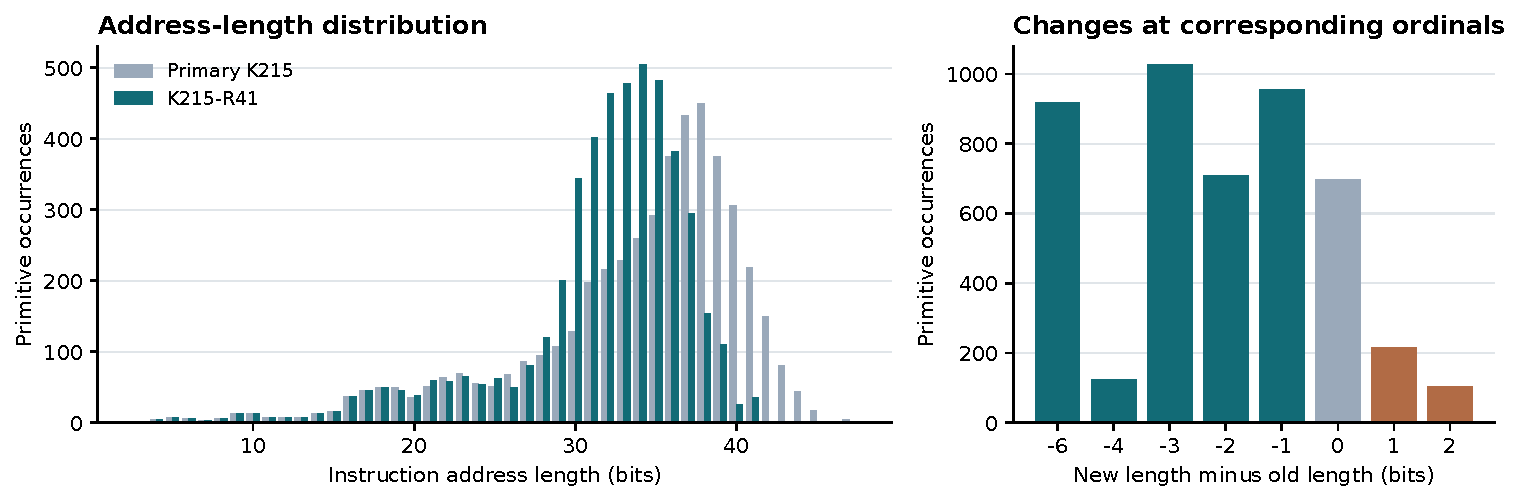
\includegraphics[width=\linewidth]{figures/address_lengths.pdf}
\caption{Static source-address measurements computed from the delivered
old and new source files. Negative changes mean shorter addresses.
These are not execution-frequency measurements.}
\label{fig:lengths}
\end{figure}

Shallower addresses do not imply uniform runtime improvement for this
engine. Matching the 6,176 symbolic primitive durations by source
ordinal and guard, every nonconstant coefficient is unchanged. The
constant term decreases in 1,427 cases, increases in 3,827 cases, and
is unchanged in 922. Individual differences range from $-12$ to $+12$;
their unweighted sum is $+15,528$. Without an execution distribution,
neither this sum nor the smaller source-address sum establishes total
runtime behavior. The lower symbolic-rule count is also a property of
the verification run, not a demonstrated speedup of the infinite
consistency search.

The useful new feature is a different physical realization with the
same calibrated program and a lower maximum address depth. It changes
the decoder contexts available for subsequent folds while retaining
the arithmetic and logical contracts. Whether those contexts permit a
214th-state deletion remains open.

% Include-only supplement: requires amsmath, amssymb.
\section{An experimental alternative: replace rejection by matrix inflation}
\label{sec:large-matrix-research}

This section gives a new source experiment and separates three claims: a
proved ordinary first-order padding lemma, an ordinary compiler proof for
an exactly specified restricted numerical calculus, and an unresolved
lower consistency reduction. It supplies no smaller accepted binary
machine. In particular, it must not be used as a second proof of the
215-state machine in the main part of this report.

\subsection{The concrete source transformation}

Use the accepted numerical constructors
\[
 P(x,y)=\frac{(x+y)(x+y+1)}2+y,\quad I(x,y)=4P(x,y),\quad
 Q_iX=4P(i,X)+2,\quad F=1,\quad T=0.
\]
The accepted AX command starts with numerical parameters
\(U=d,\ A=d+x,\ B=h+y,\ c\), where \(d,h\) are its incoming
counter and cache. Its logical rows and generalization output are left
unchanged. Immediately before the final theory bundle is constructed,
replace the matrix/private-label parameter by
\[
                         C=c+A+B+1.                 \tag{LM}
\]
Emit the existing literal bundle \(\mathrm{bundle}_{222}(A,B,C)\)
unconditionally, and clear the three parameter counters on exit. Since
\(C>A+B\), both old inequalities \(C\ne A,B\) hold automatically.
The two final equality comparisons are therefore unnecessary for these
newly emitted bundles.

The source implements (LM) with two preserving additions and one
increment. A preserving addition from register \(i\) into register 3,
using initially zero scratch register 6, first decrements \(i\) while
incrementing registers 3 and 6, then transfers register 6 back to
\(i\). Both loops terminate by a decreasing natural counter. Thus the
parameters \(A,B\) and every other register retain their exact values;
only register 3 changes, and the scratch is again zero. Each addition
has seven primitive occurrences. The old 34-occurrence final comparison
and cleanup segment is replaced by six occurrences clearing registers
3, 5, and 4. The net saving is thirteen primitive occurrences.

The deterministic source script pins the accepted K215 source hash,
retains the old first bundle factor literally after the insertion, and
checks every unchanged exterior instruction and guarded edge with two
independent control-flow resolvers. It also checks 1,728 finite addition
and cleanup interfaces. The all-natural statement follows from the loop
argument above, not from those finite probes. The source has
\[
 \begin{array}{c|r}
 \text{distinct source subtrees}&206\\
 \text{primitive occurrences}&4,738\\
 \text{guarded primitive cases}&6,155\\
 \text{maximum address depth}&46\\
 \text{maximum zero run}&6
 \end{array}
\]
with 39 newly occurring and 35 removed source subtrees. These are source
metrics, not a binary-state count. No physical allocation or blank-tape
initialization has been certified for this experiment.

\subsection{A cofinal padding lemma for ordinary first-order set theory}

Here the logical background is ordinary first-order logic, and the input
matrix is a well-formed formula of numerical code \(c\). The following
lemma does not assume that every arbitrary numerical code decodes.
Let the two public variable labels be \(a,b\), and set
\[
 s=a+b+1,\qquad e=4P(s,s)+3,\qquad t=I(e,e),\qquad
                   \widehat c=I(t,c).
\]
The code \(e\) is the explicitly well-formed atom \(v_s=v_s\).
Consequently \(t\) codes the tautology
\((v_s=v_s)\to(v_s=v_s)\), and \(\widehat c\) codes that tautology
implying the original matrix. It is therefore uniformly equivalent to
the original matrix, also under quantification and when the original
matrix is truth. No numerical zero alias is used to manufacture a
nonzero formula.

For all natural \(x,y\), \(I(x,y)\geq4(x+y)\). It follows directly
that \(\widehat c>a+b\). Also \(\widehat c>c,s\). Under the standard
native constructor coding, every variable label appearing in a positive
well-formed formula is strictly smaller than its code; this follows by
induction from the strict component bounds of each positive constructor.
Truth has no free variables. Hence the label \(\widehat c\) is fresh
for its own decoded body, including the added tautological antecedent.

Consider an ordinary first-order axiom schema whose private bound
variable can be alpha-renamed to any fresh variable, and whose matrix
occurrences respect uniform formula equivalence. The seed-K schema has
these properties: its witness, support, and subset-closure clauses are
built from the matrix by the usual logical operations. Replacing its
matrix by the padded equivalent matrix and choosing private label
\(\widehat c\) gives an allowed instance with code exceeding \(a+b\).
Replacement of equivalent formulas and alpha-conversion then recover
the original schema instance. Thus restricting the \emph{ordinary
first-order seed-K schema} to these large matrix codes preserves its
ordinary first-order deductive strength.

The qualifications in the previous paragraph matter. The actual machine
also obtains atomic quantifier vacuity from the same bundle. Ordinary
first-order logic already contains the corresponding logical principles;
the restricted numerical calculus discussed next has to recover them
from its own retained rows. The padding lemma does not supply that
recovery.

\subsection{The exact restricted calculus and its source compiler}

Define \(\mathcal D_{>}\) by retaining native truth, MP, theorem-only
GEN, all seven accepted logical rows, and every accepted dominated
\(\rho_8(A,B,c,U)\) instance with \(U\leq A\). Replace only the bundle
schema by
\[
          \mathrm{bundle}_{222}(a,b,C),\qquad C>a+b.
\]
All these are axioms of the accepted numerical calculus, so
\(\mathcal D_{>}\) is a literal subcalculus. The modified AX command
emits exactly its logical rows at the old parameters and its bundle at
\(C=c+A+B+1\). Every allowed bundle is enumerable by choosing
\(c=C-A-B-1\); the other rows remain independently selectable.

For completeness, one must repair the old reset argument: the new top
bundle is always emitted, whereas the old reset exploited a disabled
bundle. The repair uses its literal constructor shape. Every emitted
bundle is
\[
                         g=I(z,1)
\]
for some natural \(z\). Hence \(g\ne1\), and injectivity of Cantor
pairing gives \(I(g',0)\ne I(z,1)\) for every \(g'\).

Write a command-boundary state as \((t,S,d,h)\), with encoded stack
\(S\). Let \(N\) denote NIP, and put
\[
 H=\operatorname{AX}(0;0,0)N^{10},\qquad
               \operatorname{RESET}=HH\operatorname{MP}(0).
\]
After one \(H\), the state is \((g_1,S,0,t)\). The first nine NIPs
load newly emitted constructor codes, none equal to 1; the tenth loads
the old current value only on exit, without testing it. The second AX
overwrites that cache before another NIP. After the second \(H\), the
state is \((g_2,S,0,g_1)\). The final MP checks
\(I(g_2,0)=g_1\), which is impossible by the displayed constructor
shapes. Therefore RESET returns exactly \((0,S,0,0)\) from every
numerical incoming tuple, without an early halt. This also preserves a
stack whose protected old entries are arbitrary or equal to falsity.
The identity \(P(0,0)=0\) causes no problem: pairing and unpairing are
used literally and the old stack is never inspected.

All the usual strong compiler blocks now work with this RESET. A block
for a theorem \(X\), from an arbitrary work tuple and protected stack
\(S\), either halts or returns \((X,S,0,0)\). For row selection, after
RESET and the usual parameter setter \(J(U)\), execute AX and
\(N^j\operatorname{DROP}N^{11-j}\) to select row \(j\),
\(1\leq j\leq9\). The ninth row is the cached generalization.
The inserted top bundle is merely pushed and discarded during selection;
its non-falsity constructor shape is sufficient, and it need not be zero.
For a desired bundle with \(C>a+b\), use
\[
 \operatorname{RESET};\operatorname{AX}(C-a-b-1;a,b);N^{10}.
\]
Here the last two AX arguments specify the increments producing
\(A=a,B=b\); their actual wire order remains the accepted YX order.
The GEN block and the original MP-premise block preserve their same
stack equations after this reset replacement. In the MP block, the
extra top bundle is discarded before the protected success zero; every
cache test is either a generated non-falsity code or a derived premise,
so an early halt is permitted by the strong contract.

Induction on a \(\mathcal D_{>}\) derivation therefore supplies finite
compiler blocks. Append DROP, NIP, NIP to a block for code 1 to obtain a
halting block. The unchanged number scheduler is complete for every
finite initial cutoff: an arbitrary large first AX selector, followed
by RESET and a fixed refutation block, gives a cofinal family of
candidate numbers. Soundness is the original theorem/stack invariant,
now with the smaller bundle schema. These are ordinary, all-natural
source-level arguments; they are not a physical runtime theorem.

\subsection{The unresolved lower bridge}

The large-matrix bundle also supplies only the following atomic-vacuity
instances:
\[
          R(a,b)\longrightarrow Q_C R(a,b),\qquad C>a+b.
\]
The accepted numerical proof system used this bundle to obtain vacuity
for every \(C\ne a,b\). Neither semantic matrix padding nor an appeal
to ordinary first-order completeness can silently fill that gap.
A proof of the lower reduction must work in \(\mathcal D_{>}\) and
recover enough of the missing logical interface, or give a different
finite-refutation translation that bypasses it.

Accordingly, the current conclusions are deliberately limited: the
ordinary seed-K schema restriction is harmless under a full ordinary
first-order background; the modified source searches exactly the
specified restricted numerical calculus under the inherited arithmetic
macro contracts and the reset proof above; and that numerical calculus
is a subcalculus of the accepted one. Its equivalence in consistency to
ZFC, and any smaller binary realization, remain open. The source and
its audit are included to make this next experiment concrete.


\section{Other encoding experiments and their exact boundaries}
\label{sec:negative}

\subsection{A maximum-zero-run-five source}

The current interpreter's source addresses have maximum zero run six.
A source search produced an exact graph-equivalent alternative with
maximum zero run five, 4,751 primitive occurrences, depth 45, and 205
distinct subtrees. Starting from a layout with only two remaining
six-zero addresses, one closed rotation of a repeated 160-leaf factor
with factor sizes $(52,28,80)$ removes them. The exact source and a
portable finite equivalence check are supplied in \file{research/source/}.

This exposes a concrete tradeoff: saving a zero-scanner stage may cost
additional decoder roles. A constrained width-256 closed-association
beam examined 76,207 distinct sources and ended with 205 as its best
DAG count. The restricted role-pool allocator could not place that
source: its 108 new roles had at most roughly 89 compatible candidate
states per role. These observations are failures of that allocation
policy, not lower bounds for all encodings. There is no completed
smaller binary machine behind this source-only result.

\subsection{Changing spare blocks: a correct engine can initialize badly}

Changing native row $198/0$ from $1L40$ to $0L40$ changes the increment
engine's appended spare value from one to zero. With the corresponding
contract parameter \file{append=0}, all 6,176 primitive cases pass for
the accepted source. Other primitive effects are unchanged. This is a
concrete alternative interpreter contract, and the complete records and
a reproduction script are included in \file{research/spares/}.

Its literal blank startup is fatal to its intended use: after 78 steps
it is in state 35 at head coordinate 4, with its right exterior zero,
and $35/0=1R35$. It then moves right forever, writing ones. This is an
exact divergence proof, independent of ZFC consistency. It does not give
the intended consistency calibration. Trying all 215 existing initial
states to a 300,000-step cap finds 213 exact outward rays and two
bounded unresolved runs, not a usable seed. A further bounded
one-row-bootstrap search finds no accepted repair. None of these
bounded failures proves that every possible repair is impossible.

\subsection{Exchanging the enumeration and list registers}

The direct exchange of logical registers $N$ and $L$ also gives a
215-state interpreter passing all 6,176 arbitrary-natural cases, for
its exchanged source. Its literal start-0 blank run halts after 15,607
steps. The corresponding commands120 and composed variants halt after
5,151 and 15,613 steps. The engine theorem by itself therefore cannot
justify treating these machines as consistency searches.

For the primary exchange, a check of all 215 existing start states to
one million transitions per state finds 210 exact outward rays, three
halts, and two unresolved bounded runs (starts 66 and 94), with no safe
root seed found. Its positive control recovers the accepted primary
seed at exactly 95,714 steps. The unresolved runs remain unresolved.

\subsection{Why the searches are not minimality proofs}

An abstract closed-source beam visited 319,346 distinct sources before
its time cap. It reached depth 40 at 202 subtrees, but the inherited
restricted allocator could not realize that abstract source. The
successful physical search visited 2,201 distinct tables through 5,624
proposals and reached the depth-41 layout delivered here. Contextual
helper-fold screens on 32 earlier depth-44/45 rotated tables explored a
bounded last-four-context family with bounded local paths and found no new
surviving fold; positive and negative controls are included.

These searches sample specific transformation families. They do not
rule out a different source language, a different proof calculus,
context-sensitive sharing outside the checked families, a new
initialization, or a 214-state machine. Search logs and experiments
are deliberately separated from the accepted exact-table proof.

\section{Next steps suggested by the evidence}

Three directions are concrete enough to pursue without losing the
current proof boundary. First, use the new physical layout as input
to an allocator that reasons jointly about engine contexts and source
roles. Pure DAG size misses these interactions. A viable deletion must
still pass the exact quantified runtime and blank-seed checks.

Second, the zero-run-five source provides a fixed target for a more
permissive allocation strategy. It makes the scanner/decoder tradeoff
explicit; it does not yet improve the number of states. A useful
optimization objective should include decoder role sharing, zero-scan
length, and initialization constraints at the same time.

Third, matrix inflation attacks a different cost: replacing a rejection
test by construction of an automatically valid parameter. Its ordinary
first-order padding lemma and its repaired raw-code reset block are
proved in the preceding supplement. The exact missing task is to
recover or bypass the restricted numerical atomic-vacuity interface.
Completing that lower consistency reduction would turn the thirteen-leaf
source saving into an admissible formalism change; binary allocation
would remain a further independent obligation. It would be incorrect
to treat the ordinary padding lemma alone as solving that task.

\section{Reproduction and proof responsibilities}

Python 3.10 or later is sufficient for the main machine checks; they use
the standard library only. Run with assertions enabled, not with
\file{python -O}. From the packet root:
\begin{lstlisting}
# Finite reconstruction, graph differences, and exact blank seed:
python3 code/verify.py --quick --output /tmp/k215r-quick-new

# The same checks plus a fresh full symbolic runtime derivation:
python3 code/verify.py --output /tmp/k215r-full-new

# Independent reconstruction and audit of the saved actual records:
python3 code/review_depth41.py --packet . \
  --output /tmp/k215r-independent-new.json
\end{lstlisting}
Use a fresh output directory for each main verifier invocation. The
saved complete symbolic run took about 134 seconds in the research
environment; this is a reproduction observation, not a hardware-neutral
benchmark. The independent finite review has already been run on the
delivered ten-step recipe and actual completed records.

The responsibilities are deliberately separated:
\begin{enumerate}
\item \file{code/reconstruct_rotated.py} builds the exact source and
  tables from the pinned baseline and ten rotations, checking local
  closure, whole source graphs, and decoder prefixes.
\item \file{code/verify.py} binds file identities, reconstructs the
  candidate, checks graph distinctness and the complete calibrated
  blank prefix, and by default executes the symbolic checker anew.
\item \file{runtime/validate_native.py} and its unchanged inherited
  helpers derive the quantified binary primitive contracts. They do
  not prove numerical-calculus calibration.
\item \file{code/review_depth41.py} independently reconstructs the
  finite source/table result and audits the saved actual runtime and
  initialization evidence. It does not substitute receipt inspection
  for running the symbolic induction checker.
\item The pinned predecessor proofs supply the compact-calculus/ZFC
  reduction and command completeness. This report explains their
  composition with the new exact-table obligations.
\end{enumerate}

Build the PDF with two runs of \file{pdflatex K215_Rebalanced_Report.tex}.
The figure PDF is included, so matplotlib is unnecessary for that
build; \file{code/plot_addresses.py} regenerates it if desired.
The included \file{SHA256SUMS} covers the deliverables and research
supplements. The archived runtime and startup JSON files are gzip
compressed without changing their data. Main checks work offline.

\appendix
\section{The complete native patch}
\label{app:patch}

Replace the following nineteen rows of the pinned primary native table.
All write bits equal the read bit and all moves in this patch are right.
No working state is added or deleted. The archive contains all 430 rows
of both final presentations, so the patch is not required to use the
machine.

\begin{center}
\begin{tabular}{rrrrr@{\qquad\qquad}rrrrr}
\toprule
State & Read & Write & Move & Next & State & Read & Write & Move & Next\\
\midrule
101&1&1&R&153&188&0&0&R&181\\
132&0&0&R&180&188&1&1&R&177\\
132&1&1&R&158&203&0&0&R&222\\
142&0&0&R&143&203&1&1&R&223\\
142&1&1&R&147&204&0&0&R&207\\
143&0&0&R&90 &204&1&1&R&101\\
143&1&1&R&213&215&0&0&R&112\\
177&1&1&R&89 &215&1&1&R&172\\
181&0&0&R&151&223&1&1&R&215\\
181&1&1&R&204&&&&&\\
\bottomrule
\end{tabular}
\end{center}

\clearpage
\section{Attribution and references}

The new work consists of the selected physical reassociations, the
independent finite review, research experiments, and their exposition.
The existing interpreter, compact logical calculus, arithmetic/source
compiler, baseline source, runtime induction machinery, and predecessor
proofs retain their original attribution. In particular, the package
preserves the ProveIt, Wade/compiler, original machine, and normalized
source notices supplied with K215. The compact K-theory development
and earlier consistency-machine work are not new claims of this packet.
See \file{NOTICE.md} and \file{licenses/} for the exact retained notices.

\begingroup
\small\raggedright
\begin{thebibliography}{9}
\bibitem{primary}
V. Reshetnikov et al., ProveIt, \emph{candidate-k215: ordinary proof and
accepted exact-table artifacts}, pinned commit
\file{75716498437bfc7291d5900cab2983a11fd54bac}.
\href{https://github.com/VladimirReshetnikov/ProveIt/blob/75716498437bfc7291d5900cab2983a11fd54bac/Computability/BusyBeaver/Research/ZFC/candidate-k215/proof.md}{Pinned upstream proof};
local copy \file{baseline/proof-upstream.md}.
\bibitem{permuted}
ProveIt, \emph{Ordinary proof for the command-permutation alternatives},
same pinned commit, \file{candidate-k216/alternatives/permuted/proof.md}.
\href{https://github.com/VladimirReshetnikov/ProveIt/blob/75716498437bfc7291d5900cab2983a11fd54bac/Computability/BusyBeaver/Research/ZFC/candidate-k216/alternatives/permuted/proof.md}{Pinned upstream proof};
local copy \file{baseline/command-calibration-upstream.md}.
\bibitem{dominated}
ProveIt, \emph{Ordinary proof boundary of the dominated-rho8 machine},
same pinned commit, \file{candidate-k218/alternatives/dominated/proof.md}.
\href{https://github.com/VladimirReshetnikov/ProveIt/blob/75716498437bfc7291d5900cab2983a11fd54bac/Computability/BusyBeaver/Research/ZFC/candidate-k218/alternatives/dominated/proof.md}{Pinned upstream proof};
local copy \file{baseline/dominated-calibration-upstream.md}.
\bibitem{artifacts}
This packet, \file{verification/construction.json},
\file{verification/runtime/runtime.json},
\file{verification/independent_review.json}, and the accompanying
unchanged literal inputs and executable checkers. These are the
primary evidence for all new numerical measurements in this report.
\end{thebibliography}
\endgroup
\end{document}
